%%%%%%%%%%%%%%%%%%%%%%%%%%%%%%%%%%%%%%%%%
% NIWeek 2014 Poster by T. Reveyrand
% www.microwave.fr
% http://www.microwave.fr/LaTeX.html
% ---------------------------------------
%
% Original template created by:
% Brian Amberg (baposter@brian-amberg.de)
%
% This template has been downloaded from:
% http://www.LaTeXTemplates.com
%
% License:
% CC BY-NC-SA 3.0 (http://creativecommons.org/licenses/by-nc-sa/3.0/)
%
%%%%%%%%%%%%%%%%%%%%%%%%%%%%%%%%%%%%%%%%%

%----------------------------------------------------------------------------------------
%   PACKAGES AND OTHER DOCUMENT CONFIGURATIONS
%----------------------------------------------------------------------------------------

\documentclass[a0paper,portrait]{baposter}

\usepackage[font=small,labelfont=bf]{caption} % Required for specifying captions to tables and figures
\usepackage{booktabs} % Horizontal rules in tables
\usepackage{relsize} % Used for making text smaller in some places
\usepackage{amsmath,amsfonts,amssymb,amsthm} % Math packages
\usepackage{eqparbox}
\usepackage{textcomp}
\usepackage{caption}
\usepackage{subcaption}
\usepackage{graphicx}
\usepackage{listings}
\usepackage{enumitem}
\usepackage{pgf}
\usepackage{tikz}
\usetikzlibrary{positioning}
\usepackage[utf8]{inputenc}
\usetikzlibrary{arrows,automata}
\usetikzlibrary{positioning}
\usepackage{multirow}
\usepackage{array}
\newcolumntype{P}[1]{>{\centering\arraybackslash}p{#1}}
\captionsetup[figure]{labelformat=empty}

\graphicspath{{figures/}} % Directory in which figures are stored

 \definecolor{bordercol}{RGB}{40,40,40} % Border color of content boxes
 \definecolor{headercol1}{RGB}{186,215,230} % Background color for the header in the content boxes (left side)
 \definecolor{headercol2}{RGB}{120,120,120} % Background color for the header in the content boxes (right side)
 \definecolor{headerfontcol}{RGB}{0,0,0} % Text color for the header text in the content boxes
 \definecolor{boxcolor}{RGB}{210,235,250} % Background color for the content in the content boxes


\tikzset{
    state/.style={
           rectangle,
           rounded corners,
           draw=black, very thick,
           minimum height=2em,
           inner sep=3pt,
           text centered,
           },
}

\begin{document}
\setlength{\fboxsep}{0pt}

\background{ % Set the background to an image (background.pdf)
\begin{tikzpicture}[remember picture,overlay]
\draw (current page.north west)+(-2em,2em) node[anchor=north west]
{
\includegraphics[height=1.1\textheight]{background}};
\end{tikzpicture}
}

\begin{poster}{
grid=false,
columns=4,
borderColor=bordercol, % Border color of content boxes
headerColorOne=headercol1, % Background color for the header in the content boxes (left side)
headerColorTwo=headercol2, % Background color for the header in the content boxes (right side)
headerFontColor=headerfontcol, % Text color for the header text in the content boxes
boxColorOne=boxcolor, % Background color for the content in the content boxes
headershape=roundedright, % Specify the rounded corner in the content box headers
headerfont=\Large\sf\bf, % Font modifiers for the text in the content box headers
textborder=rectangle,
background=none,
headerborder=open, % Change to closed for a line under the content box headers
boxshade=plain
}
{
\includegraphics[width=4cm]{BiATA2020.png}}
%
%----------------------------------------------------------------------------------------
%   TITLE AND AUTHOR NAME
%----------------------------------------------------------------------------------------
%
{ \bf  \huge {Secondary Structure Prediction by Combination of Formal Grammars and Neural Networks} }  % Poster title
{\vspace{0.3em} \smaller \textbf{Polina Lunina$^1$}, Dmitry Kutlenkov$^1$, Semyon Grigorev$^1$ \\  % Author names
\smaller \it $^1${Saint Petersburg State University, JetBrains Reserach, St. Petersburg, Russia } \\ % Author email addresses
\smaller  {\textbf{E-mail:} lunina\_polina@mail.ru, kutlenkov.dmitri@gmail.com, semyon.grigorev@jetbrains.com}}
{
\includegraphics[width=3cm]{SPbGU_Logo.png}} % University/lab logo


%----------------------------------------------------------------------------------------
%   INTRODUCTION
%----------------------------------------------------------------------------------------
\headerbox {Introduction}{name=introduction,column=0,row=0, span=2}{

Secondary structure is known to have a crucial impact on the RNA molecule functioning, therefore, development of the algorithms for secondary structure modeling and prediction is a fundamental task in computational genomics.
An approach for sequences secondary structure analysis by combination of formal grammars and neural networks was proposed in ~\cite{grigorev2019composition}. We encode stems of secondary structure by means of context-free grammar, extract them by parsing algorithm and then process the parsing provided data by neural network. In this work, we apply this approach to RNA secondary structure prediction problem.

\vspace{-0.5mm}
}

\headerbox {Research Motivation}{name=rq,column=2,row=0, span=2}{

Secondary structure can be described as composition of stems having different heights and loop sizes. We use context-free grammar to encode the most common kinds of stems and parsing algorithm to find the subsequences of sequence that should fold to such stems. 
Parsing matrix represents all the theoretically possible stems in some sequence in terms of grammar, but the real secondary structure is more complex than that. Therefore, parsing matrices require further processing and we propose using neural network to handle them in order to generate an actual secondary structure.

}

\headerbox{Solution Overview}{name=solution,span=4,column=0,row=1,below=introduction}{
  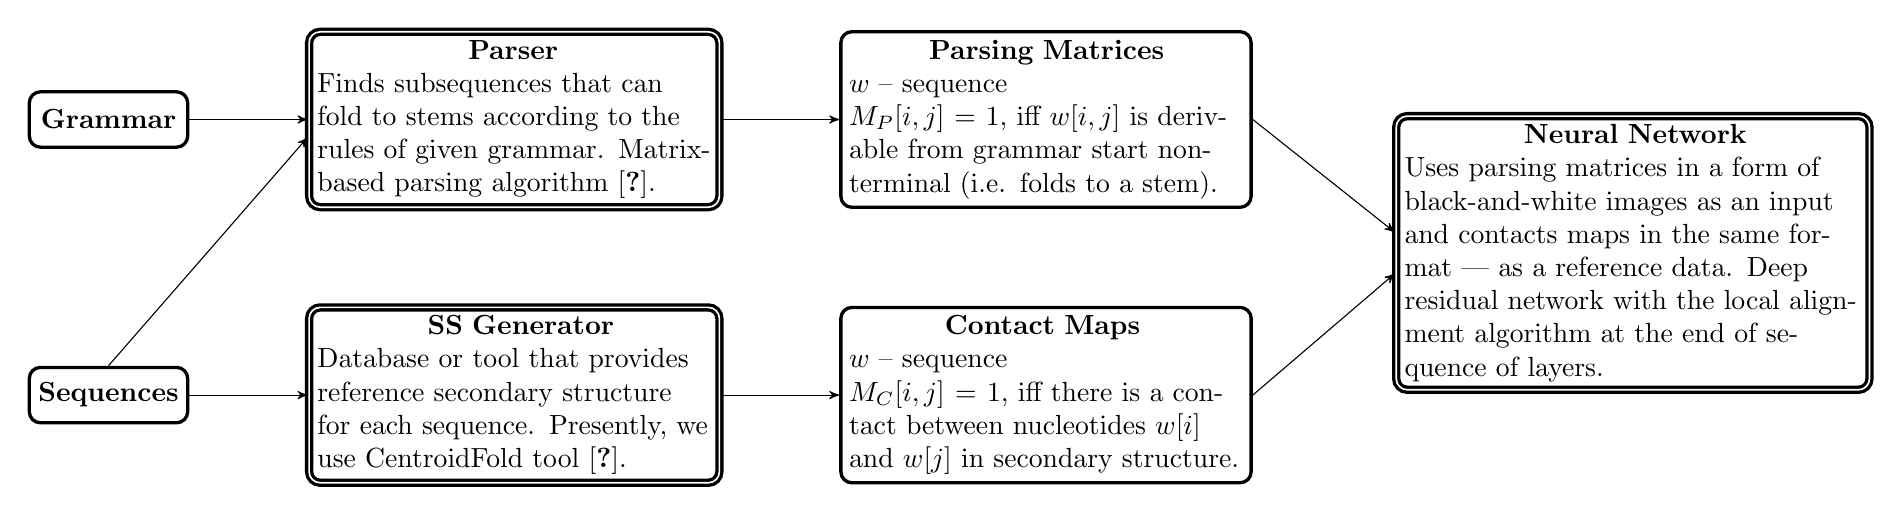
\begin{tikzpicture}[->,>=stealth']
  \node[state,
        align = center,
        text width = 1.8cm] (grm)
   {
   \textbf{Grammar}
   };

  \node[state,
        below of=grm,
        node distance=3.5cm,
        align = center,
        text width = 1.8cm] (sqs)
   {
   \textbf{Sequences}
   };

  \node[state,
        right = 1.5cm of grm,
        align = left,
        double,
        text width = 5.0cm](parser)
  {
\textbf{\hspace{18mm} Parser}\\
Finds subsequences that can fold to stems according to the rules of given grammar.
Matrix-based parsing algorithm~\cite{Azimov:2018:CPQ:3210259.3210264}.
};
  
  \node[state,
        right = 1.5cm of sqs,
        align = left,
        double,
        text width = 5.0cm](pred)
  {
  \textbf{\hspace{14mm}SS Generator} \\
  Database or tool that provides reference secondary structure for each sequence. Presently, we use CentroidFold tool~\cite{hamada2009prediction}.
  };

  \node[state,
        right = 1.5cm of parser,
        align = left,
        text width = 5.0cm] (mtrx1)
  {
\textbf{\hspace{9mm} Parsing Matrices}\\
$w$ -- sequence \\ $M_P [i,j] = 1$, iff $w[i,j]$ is derivable from grammar start nonterminal (i.e. folds to a stem).
};

  \node[state,
        right = 1.5cm of pred,
        align = left,
        text width = 5.0cm](mtrx2)
  {
  \textbf{\hspace{11mm} Contact Maps}\\
  $w$ -- sequence \\ $M_C [i,j] = 1$, iff there is a contact between nucleotides $w[i]$ and $w[j]$ in secondary structure.
 };

 
   \node[state,
        below right = -1.2cm and 1.8cm of mtrx1,
        align = left,
        double,
        text width = 5.8cm](nn)
  {
  \textbf{\hspace{14mm} Neural Network}\\
Uses parsing matrices in a form of black-and-white images as an input and contacts maps in the same format --- as a reference data. Deep residual network with the local alignment algorithm at the end of sequence of layers.
 };
 
  \path (grm) edge (parser)
  (sqs.north) edge (parser.-175)
  (sqs) edge (pred)
  (parser) edge (mtrx1)
  (pred) edge (mtrx2)
  (mtrx1.east) edge (nn.-185)
  (mtrx2.east) edge (nn.-175)
   ;
  \end{tikzpicture}
  \vspace{-2mm}
}

\headerbox {Example}{name=example, column=0, span=2, below=solution}{

\centering
\begin{subfigure}{.3\textwidth}
  \centering
  \fbox{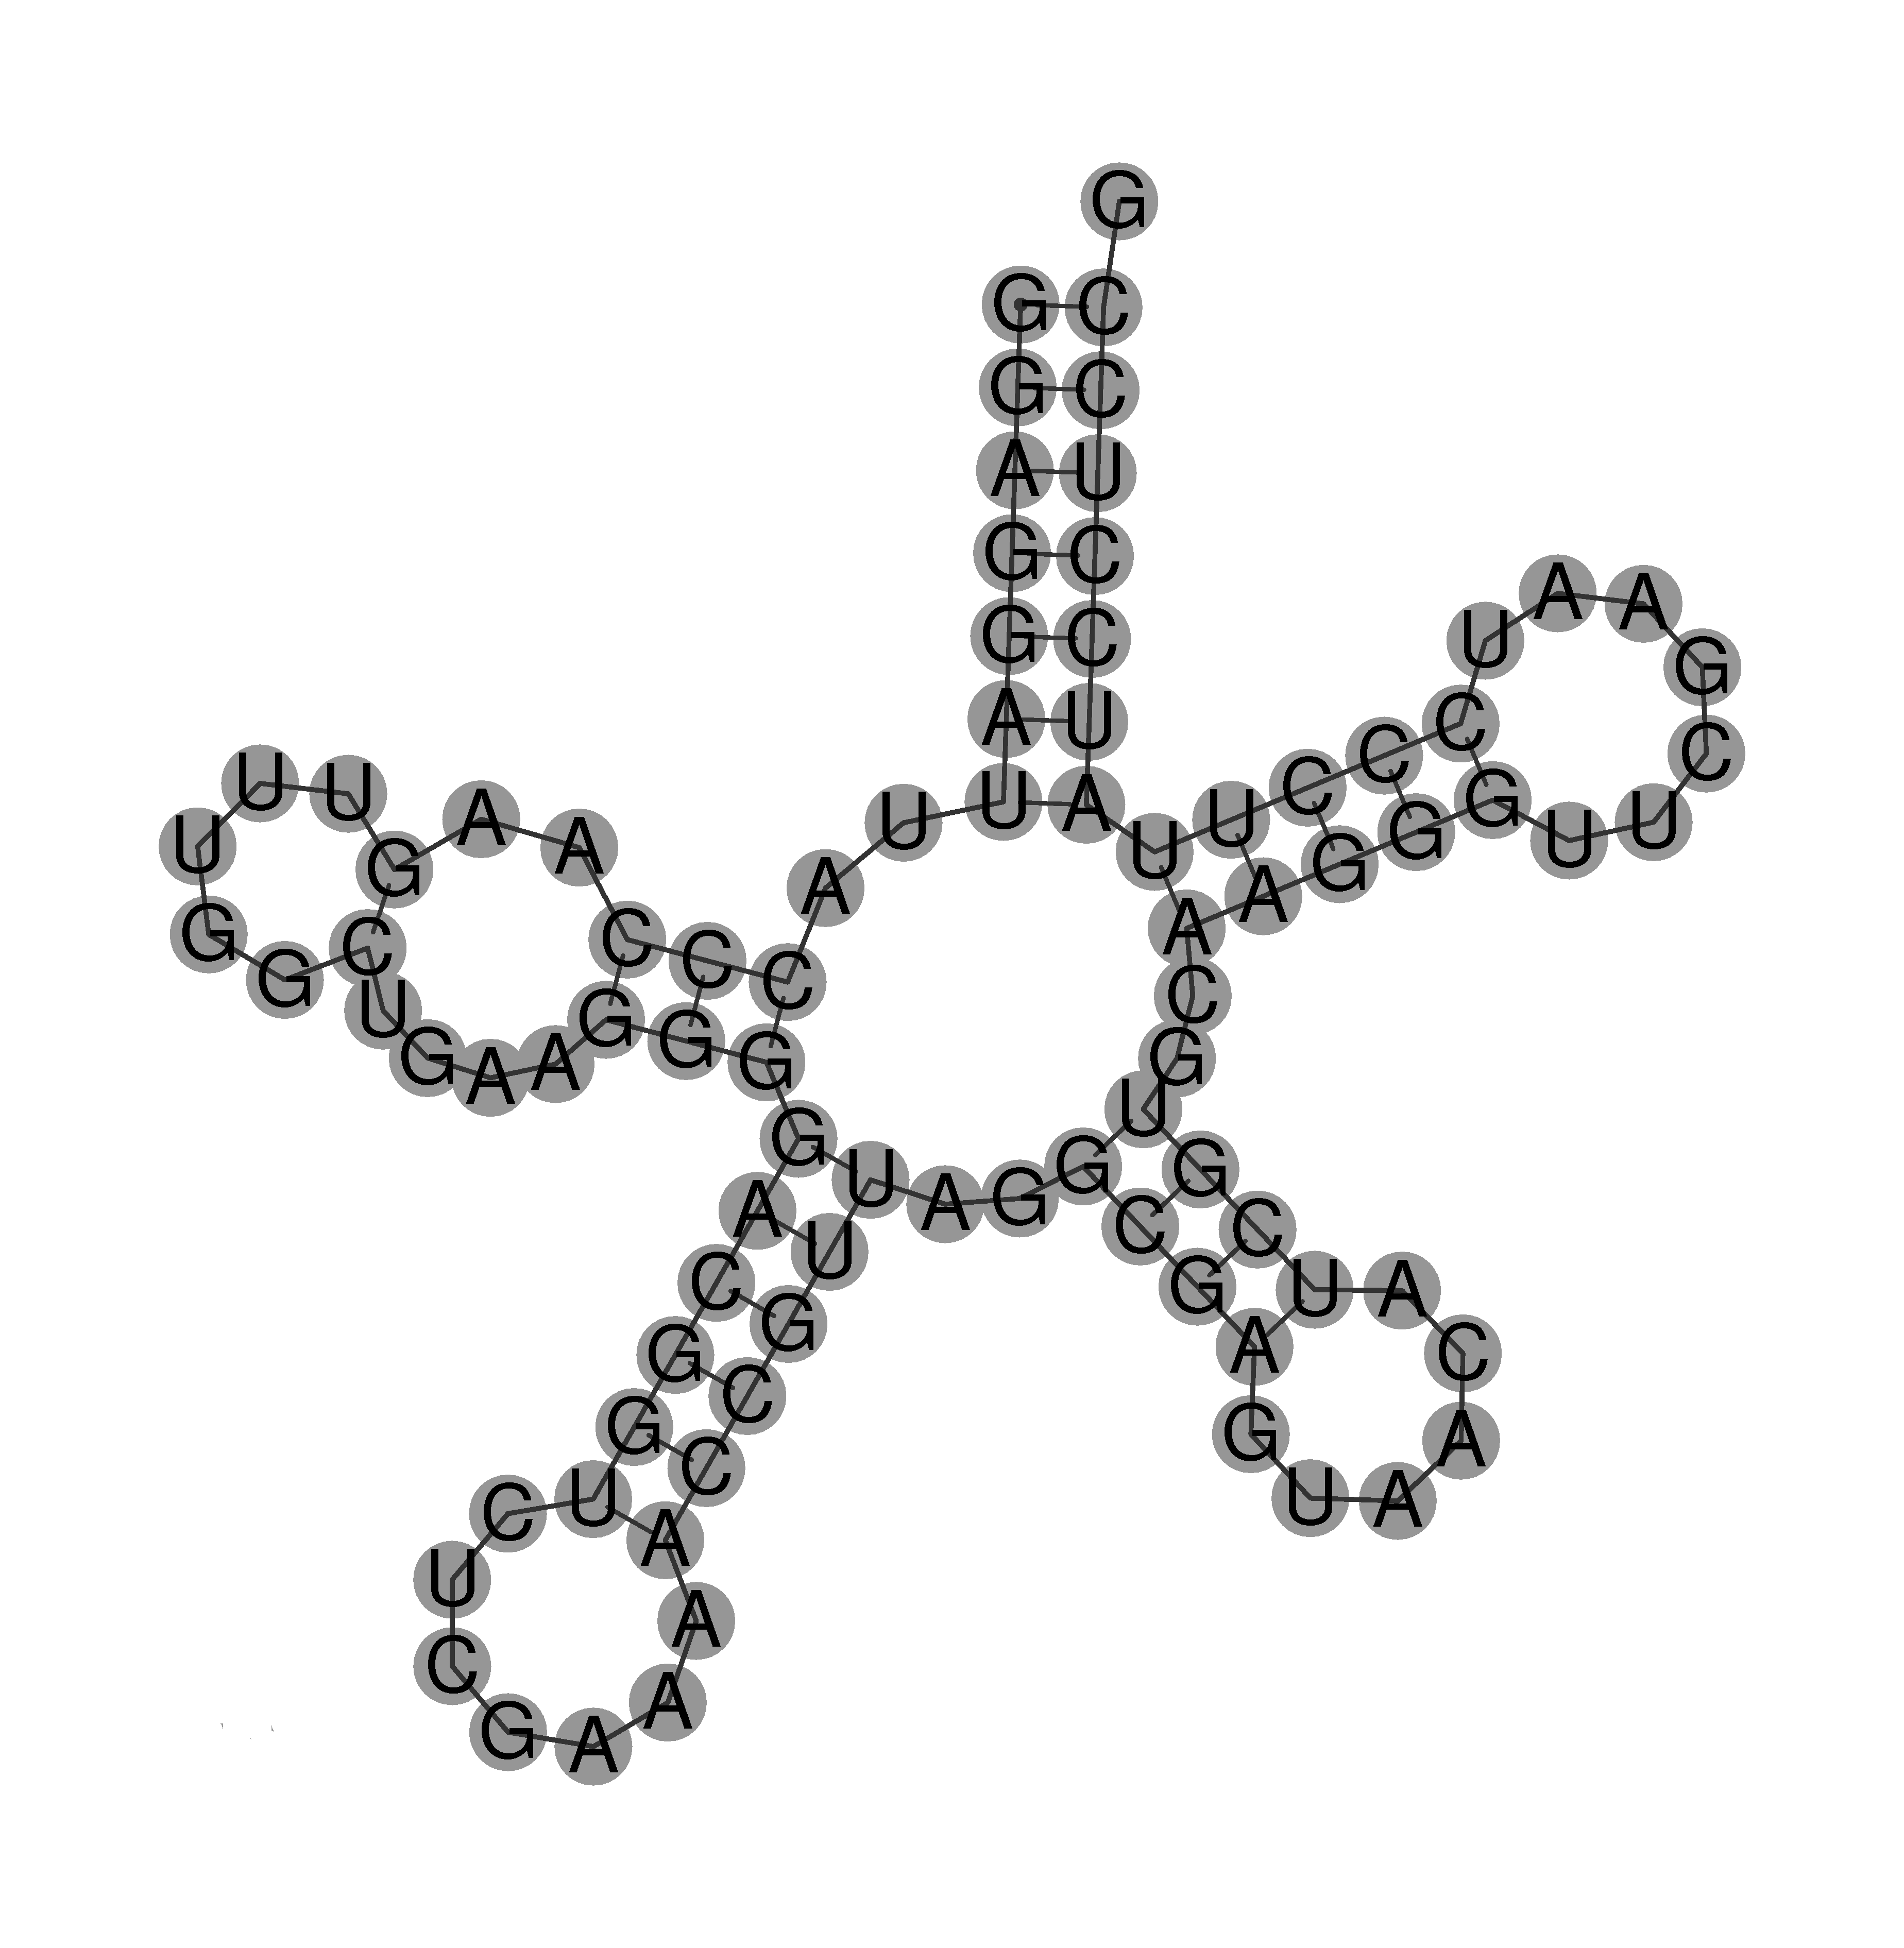
\includegraphics[width=.8\linewidth]{figures/structure.png}}
  \captionof{figure}{Secondary structure}
\end{subfigure}%
\begin{subfigure}{.3\textwidth}
  \centering
  \fbox{
\includegraphics[width=.8\linewidth]{figures/etalon.png}}
  \captionof{figure}{Contact map}
\end{subfigure}
\begin{subfigure}{.3\textwidth}
  \centering
  \fbox{
\includegraphics[width=.8\linewidth]{figures/parsed.png}}
  \captionof{figure}{Parsing matrix}
\end{subfigure}
 \vspace{0.5mm}
}

\headerbox {Metrics}{name=metrics, column=2, span=2, below=solution}{

Consider $TW$ (true white), $TB$ (true black), $FW$ (false white) and $FB$ (false black) as amounts of correctly and incorrectly predicted pixels of each color for all images.

\begin{itemize}
    \item $Precision = \frac{TW}{TW + FW}$ 
    \item $Recall = \frac{TW}{TW + FB}$ 
    \item $F1$ $score = 2 * \frac{Precision * Recall}{Precision + Recall}$ 
\end{itemize}


}


\headerbox {Results}{name=results, column=0, row=0, span=2, below=example}{

We took sequences from RnaCentral~\cite{rnacentral} database with 70\%:10\%:20\% split and trained models on several datasets with fixed sequences length interval with and without alignment.

\vspace{4mm}
\begin{tabular}{|P{1.4cm}|P{1.4cm}|P{1.4cm}|P{1.4cm}|P{1.4cm}|P{1.4cm}|}
\hline
Length & Samples & Alignment & Precision & Recall & F1 score \\ \hline \hline
\multirow{2}{*}{90} & \multirow{2}{*}{26511} & $\times$ & 67\% & 75\% & 68\% \\ \cline{3-6} 
 &  & \checkmark & 80\% & 66\% & 70\% \\ \hline \hline
\multirow{2}{*}{88-90} & \multirow{2}{*}{77976} & $\times$ & 66\% & 78\% & 69\% \\ \cline{3-6} 
 &  & \checkmark & 81\% & 62\% & 68\% \\ \hline \hline
\multirow{2}{*}{50-90} & \multirow{2}{*}{141835} & $\times$ & 60\% & 72\% & 63\% \\ \cline{3-6} 
 &  & \checkmark & 71\% & 61\% & 63\% \\ \hline
\end{tabular}

\vspace{4mm}
We can make the following conclusions.

\begin{itemize}
    \item The smaller the window size, the more accurate the model.
    \item Alignment significantly improves precision of neural networks due to removing the contacts that break the secondary structure.
    \item From the other hand, it decreases recall, probably because it also removes a part of necessary information.
    \item So, our approach is applicable to secondary structure analysis problem, but further research is required.
\end{itemize}

}


\headerbox {Future Research}
{name=fr, column=2, below=metrics, span=2}
{
\begin{itemize}
\item Improvement of prediction accuracy.
\item Experiments on structures with pseudoknots and corresponding adaptation of the alignment algorithm.
\item Building a model that predicts secondary structure for sequences of arbitrary length.
\item More accurate choice of the reference data source.
\end{itemize}
}

%----------------------------------------------------------------------------------------
%   REFERENCES
%----------------------------------------------------------------------------------------

\headerbox {References}
{name=ref,column=2,span=2, below=fr}
{
\smaller % Reduce the font size in this block
\renewcommand{\section}[2]{\vskip 0.05em} % Get rid of the default "References" section title
%\nocite{*} % Insert publications even if they are not cited in the poster

\bibliographystyle{unsrt}
%\bibliographystyle{IEEEtran}
\bibliography{biblio} % Use biblio.bib as the bibliography file
}


\headerbox {Acknowledgments}{name=ack,column=2,span=2,below=ref}{
The research was supported by the Russian Science Foundation grant 

18-11-00100 and a grant from JetBrains Research.
\vspace{0.8mm}
}

\headerbox {Information}{name=info,column=0,span=2,below=results}{

\url{https://github.com/LuninaPolina/SecondaryStructureAnalyzer}.

\url{https://github.com/SacredArrow/Secondary\_structure\_public}.
}

\end{poster}

\end{document}
